% !eX root = ../tfm.tex
%! TEX root = ../tfm.tex

\begin{comment}
Aportar detalles del proceso de desarrollo incluyendo fases e hitos del proceso, diagramas representativos de la arquitectura y funcionamiento, capturas de pantalla para ilustrar el funcionamiento, etc.
\end{comment}

Tras un primer contacto con los componentes escogidos para implementar la aplicación en el capítulo anterior nos enfrentamos al desarrollo de la plataforma final. Empezaremos recuperando la base de datos \textit{Sisfall} como mencionamos en el capítulo de requisitos (Sección \ref{sec:req:bases_datos}) para implementar un prototipo del algoritmo, lo describiremos, analizaremos los resultados y compararemos con otros métodos ya existentes.

Con el modelo validado nos centraremos en optimizarlo para mejorar el consumo de recursos de cara al siguiente paso: implementar el sistema final. Explicaremos en la estructura del sistema cliente-servidor escogida y entraremos en detalle en el estudio y análisis de la aplicación para dispositivos llevables presentada. Estudiaremos la arquitectura, interfaz de uso y rendimiento antes de abordar, en el capítulo siguiente, la idoneidad y <como de bien se adapta> a los requisitos previamente definidios.

\section{Modelo y Algoritmo de iFell}\label{sec:imp:model}

\subsection{Algoritmo}\label{sub:imp:model:algoritmo}

Con el fin de buscar un equilibrio entre capacidad de detección y requisitos del sistema, optamos por un algoritmo híbrido con dos modelos (uno analítico y otro basado en redes recurrentes), tal y como se presenta en la figura \ref{fig:ifell:algoritmo}. Al utilizar dos etapas permite mantener el costoso modelo neuronal aletargado a la espera de un evento del modelo analítico. Este modelo, más simple, apenas consiste de un comparador, puede ejecutarse sin problema de forma continua sin tener un impacto notable en la duración de la batería del sistema.

\figura[0.5]{deteccionFlujo}{fig:ifell:algoritmo}{Algoritmo de detección de caídas de iFell}

Justificamos ya en la sección \ref{sec:req:modelos} la necesidad de usar modelos que no analicen la postura, posición o inclinación del sensor debido a la falta de coherencia entre la posición del sensor respecto la del cuerpo por su situación en la muñeca. Este factor, que tendrá un impacto en la calidad del modelo obtenido infiere a la vez de mayor simplicidad y facilitará su posterior uso en sistemas embebidos.

\subsection{Modelo Analítico: Bourke2006}\label{sub:imp:model:analitico}

Presentado por \citeA{Bourke2006} es un algoritmo simple que al no requerir más que del módulo del vector aceleración permite ser usado en nuestro sistema. Usando dos cotas de detección consecutivas (una cota inferior para detectar valles en la aceleración y una superior para la detección del posterior pico como se muestra en la figura\ref{fig:bourke_thresholds}) permite identificar caídas basándose en la forma característica que sigue la aceleración del cuerpo en estos eventos.

Como el resto de modelos analíticos aplicados a la detección de caídas tiene la gran ventaja de ser computacionalmente simple. Su mayor contraprestación es la dificultad de balancear las métricas de Especificidad y Sensibilidad. Al basarse en niveles o cotas, podemos aumentar la sensibilidad situando el nivel de estas de manera que la sensibilidad llegue al 100\%, como requiere el algoritmo por definición, aunque afectará a la especificidad negativamente \cite{Aziz2017}. 

En nuestro algoritmo general, el modelo analítico es similar a una capa de gestión de la atención del modelo RNN. Es por esta razón que la baja especificidad  no resulta un problema ya que lo que nos interesa es que esta etapa tenga una sensibilidad próxima al 100\%. El dispositivo captura información de la aceleración en 3 ejes con una medida máxima de $9G$ y a una frecuencia de muestreo $f_m=50Hz$ \todo{seguro?}. Esta medida la convertimos en el módulo de la aceleración ($|\vec{A}| = |\sqrt{a_{x}^2+a_{y}^2+a_{z}^2}|$).:wa En concreto, comparamos el valor absoluto de la diferencia de dos mediciones consecutivas de la aceleración y comparamos con un umbral de referencia.
\[
ModeloAnalitico\rightarrow |SVTot_n - SVTot_{n-1}|\geq A_{umbral}
\]


Aunque ya hemos presentado los resultados de diferentes estudios que proporcionan valores para las cotas \textit{LFT} y \textit{UFT} del modelo (tabla \ref{tab:bourke_threshold_values}) también hemos comprobado la alta variabilidad de resultados según el conjunto de datos usado. Por esa razón, al no disponer de un estudio que analizase este modelo sobre la base de datos usada, calcularemos los valores usando las muestras de SisFall y analizaremos el comportamiento del modelo.

\subsubsection{Preprocesado de la base de datos}

Para acortar las distancias entre los resultados obtenidos en la simulación con los esperados sobre el dispositivo real realizamos un tratamiento previo de los datos para submuestrear a 25KHz.


\paragraph{Filtrado IIR}

Previo al subsampleado de la señal optamos por realizar un filtrado paso bajo respecto a la frecuencia de corte de Nyquist para señales muestreadas a 25Hz ($f_c=\frac{25}{2}=12,5$). Usaremos un filtro IIR de primer orden, con función de transferencia $H(z)$:

\[
  y_n = \alpha x_n + (1-\alpha) y_{n-1}
\]

%comment = \alpha\times x_n + \(1-\alpha\)\times y_{n-1}

\[
  H(z) = \frac{\alpha}{1-(1-\alpha)z^{-1}}
\]

Donde
\begin{align*}
\alpha = \frac{\delta t}{\delta t + RC} \\
f_c= \frac{1}{2 \pi RC}
\end{align*}

Dado que posteriormente submuestrearemos la señal a 25Hz y que sabemos que en estos primeros 12Hz hay suficiente información sobre las caídas, tomamos como ya hemos dicho $f_c=12,5Hz$. Hay que tener en cuenta que al ser un filtro paso bajo no afectará a la componente continua de la gravedad. Despejando las ecuación precedentes queda:
\begin{align*}
  f_m & = 200{Hz}\\
  \delta t & = 1/f_m = 0.005s\\
  RC & =\frac{1}{2\pi f_c} = \frac{1}{2\pi12,5} = 0,5\\
  \alpha & = \frac{0.02}{0.02 + RC} = 0,015
\end{align*}

\begin{comment}
%VER https://electronics.stackexchange.com/questions/498226/calculate-cutoff-frequency-of-a-digital-iir-filter
%https://en.wikipedia.org/wiki/EWMA_chart
%https://en.wikipedia.org/wiki/Low-pass_filter#Simple_infinite_impulse_response_filter
\end{comment}

El interés de realizar un filtrado prevo al subsampleado puede observarse al compararse los resultados expuestos en la figura \ref{fig:iir} en ella se observa la destrucción de información producida por el muestreado de la señal. Se aprecia claramente como en las curvas de la figura\ref{fig:signalIIRFilter25} en que se ha muestreado la señal sin filtrado previo se ha aplanado en exceso. Resultado especialmente nocivo para nuestro modelo analítico que se basa precisamente en detectar estos picos valles.

\begin{figure}[htb!]
  \centering
  \begin{subfigure}[b]{0.96\textwidth}
      \centering
      \pincludegraphics[0.9]{FilterAndDownsample}
      \caption{Degradación de la señal con submuestreados y filtrados}
      \label{fig:downsample}
  \end{subfigure}
  \centering

  \begin{subfigure}[b]{0.48\textwidth}
      \centering
      \pincludegraphics[1.0]{SignalvsIIRFilter}
      \caption{Señal original (200Hz) y filtrada}
      \label{fig:signalIIRFilter}
  \end{subfigure}
  \hfill
  \begin{subfigure}[b]{0.48\textwidth}
      \centering
      \pincludegraphics[1.0]{SignalvsIIRFilter25Hz}
      \caption{Señal submuestreada a 25Hz y filtrada}
      \label{fig:signalIIRFilter25}
  \end{subfigure}
  \caption{\label{fig:iir}  Efecto del filtro IIR y submuestreado en la señal}
\end{figure}

\paragraph{Submuestreado a 25Hz}

La base de datos SisFall usa un muestreado a 200Hz, el reloj elegido como soporte admite únicamente un muestreado a 50Hz como máximo. Sin embargo a raíz del ya expuesto resultado de \todo{falta referencia de los 12KHz} decidimos reducir el muestreado hasta los 25Hz, que por Nyquist debería ser suficiente para no destruir la información de las caídas de la señal.

El sub-muestreado se realiza tomando una muestra de cada n con $n=\frac{f_m}{f_o}=\frac{25}{200}=8$. En la figura \ref{fig:downsample} se aprecia la degradación que sufre la señal original al aplicarle el filtrado y posterior reducción de muestras. Se observa un doble efecto del filtrado: un suavizado de la señal resultante y un desfase no lineal. El suavizado enmascara parcialmente los valores pico y valle, sin embargo garantiza mayor fidelidad del resultado a la señal original: si bien se pierde la información en picos y valles, la señal mantiene mejor la estructura general. En el fondo se ha reducido el ruido de la señal ya que el filtro en la práctica actúa como un ponderador.

%\figura{FilterAndDownsample}{fig:downsample}{Efecto de filtrar y submuestrear la señal)





\begin{comment}
Los estudios siguientes demuestran que el filtrado de ruido mejora la capacidad de tratamiento posterior
Tian, T.; Sun, S.; Lin, H. Distributed fusion filter for multi-sensor systems with finite-step correlated noises. Inf. Fusion 2019, 46, 128-140.

Luego, para el caso de natación
Xiao, D.; Yu, Z.; Yi, F.; Wang, L.; Tan, C.C.; Guo, B. Smartswim: An infrastructure-free swimmer localization system based on smartphone sensors. In Proceedings of the International Conference on Smart Homes and Health Telematics, Wuhan, China, 25-27 May 2016; pp. 222-234.

decide que una promediado por ventana flotante de tamaño M es el que mejores resultados da: $G_{filter}=\frac{1}{M}\sum_{i=0}^{M}G_i$. (Explicado en Liu \cite{Liu2020} que usa este método con una DeepNN basada en capas CNN + 2xLSTM + Fully Connected + Softmax).

% \figura{capturaFlujo}{fig:capturaFlow}{Flujo de trabajo de la aplicación de captura de datos}
\end{comment}

\subsubsection{Cálculo de parámetros para el modelo Bourke}

Realizamos una primera iteración por todas las secuencias incluidas en el conjunto de datos buscando el valor de valle y de pico para cada una y agrupamos los resultados en dos categorías: \textit{actividad normal} o \textit{caída}. Posteriormente analizamos los histogramas resultantes para obtener la función de densidad de la distribución de ambos valores. Si se observa la figura \ref{fig:bourke:hist} a primera vista la capacidad de segregación entre caídas y actividades de la distribución de los picos de aceleración es mayor que la de los valles. En parte previsible dado lo compacto del rango ( 1g) comparado con el de los valores de pico que es potencialmente ilimitada, o limitado únicamente por la capacidad del sensor. Analizando los datos, en el caso de los valores de pico, el percentil 0\% de las caídas se sitúa en 4,5g que se corresponde con el percentil 23\% de las actividades: si establezco la cota de pico en 4,5g conseguimos detectar el 100\% de la caídas aunque detectemos también como tales el 73\% de las actividades normales. Este porcentaje baja hasta el 59\% si aceptamos no detectar el 1\% de las caídas poniendo la cota en 5.7g. Para el caso de los valles si queremos detectar el 100\% de las caídas debemos situar la cota en 0,97g lo que apenas filtraría el 4\% de las actividades normales, aunque mejora hasta el 27\% si aceptamos no identificar el 1\% de las caídas.

\begin{figure}[htb!]
  \centering
  \begin{subfigure}[b]{0.48\textwidth}
      \centering
      \pincludegraphics[1.1]{BourkeLowThresholdsHistogram}
      \caption{Histograma valores \textit{valle} modelo Bourke}
      \label{fig:bourke:hist:low}
  \end{subfigure}
  \hfill
  \begin{subfigure}[b]{0.48\textwidth}
      \centering
      \pincludegraphics[1.1]{BourkeUpperThresholdsHistogram}
      \caption{Histograma valores \textit{pico} modelo Bourke}
      \label{fig:bourke:hist:high}
  \end{subfigure}
  \caption{\label{fig:bourke:hist} Histogramas de valores pico y valle}
\end{figure}

Es evidente a la luz de estos datos que los resultados del clasificador sobre SisFall son mediocres. Sin embargo dada su función de mecanismo atencional y la particularidad del conjunto de datos, enfocado al estudio de caídas y con muchos eventos similares a caídas etiquetados como actividades, es un resultado esperable.


\subsubsection{Evaluación del modelo Bourke sobre SisFall}

De forma aleatoria apartamos un 20\% (901 muestras) de las muestras de SisFall como conjunto de datos de validación y usamos las 3604 restantes como conjunto de entrenamiento. Recordamos que SisFall está compuesto por 4505 muestras, 1798 de las cuales se corresponden con caídas (el 39,7\%). Las caídas están por tanto sobrerrepresentadas con respecto a su ocurrencia en la vida real.

Tomando el conjunto de datos de entrenamiento previamente filtrado y submuestreado a 25Hz, iteramos sobre los datos de la aceleración para buscar los valores de pico y valle de cada ejercicio. Para establecer las cotas, Bourke propone establecer los niveles de tal forma que el 100\% de las caídas entren dentro del espacio, consiguiendo una sensibilidad del mismo valor por definición. 

\tabla[0.4\linewidth]{tab:bourke:valores}{Valores UFT y LFT del modelo Bourke según percentil}{lllll}{
         & \multicolumn{4}{c}{Valor Percentil} \\ \cmidrule(lr){2-5}
    Cota & p. 0\%         & p. 1\% & p. 3\% & p. 10\%\\ \midrule
    UFT  & \textbf{4,16g} & 5,77g  & 6,67g  & 8,69g\\
    LFT  & \textbf{0,97g} & 0,86g  & 0,81g  & 0,68g\\
  }{3}

Este modelo tiene la desventaja de tener una especificidad muy baja. Los resultados sobre SisFall nos arrojan un valor para las cotas de 0,971g para el valle y 4,164g para el pico (en la tabla \ref{tab:bourke:valores} se presentan los resultados para otros percentiles). Con estos valores se consigue una especificidad de tan solo el 28,7\% mientras que la sensibilidad se queda en 97,2\% usando Bourke estándar (lo designaremos como modelo \textit{BourkeUL} en adelante). Repetimos el experimento iterando sobre dos variaciones del modelo de Bourke: \textit{BourkeU} que busca únicamente los casos que superan la cota de pico y \textit{BourkeL} que hace lo propio con los valles. También variamos el valor de las cotas según el porcentaje de caídas que cumplen dicha cuota en cada caso. En la figura \ref{fig:bourke_cfmatrix} se muestran las matrices de confusión y los valores de sensibilidad y especificidad para cada combinación.

\figura[0.9]{BourkeCONF_Matrix}{fig:bourke_cfmatrix}{Matrices de confusión para modelos Bourke}

Al interpretar los resultados obtenidos interesa entender principalmente la causa por la que \textit{BourkeUL} no alcanza el 100\% de sensibilidad. Lo achacamos al hecho de que para ser detectado por el modelo implementado, la caída ha de cumplir ambas cotas en una ventana deslizante de 200 muestras. El siguiente resultado, y de mayor interés para el trabajo es el buen resultado obtenido por la variante \textit{BourkeU}: Alcanza el 100\% de sensibilidad y la especificidad es la mejor de todos los modelos a igual sensibilidad (por ejemplo, si bajamos la sensibilidad hasta el 97,2\% tiene una especificidad del 43,6\%, mucho mayor que el 28,7\% de \textit{BourkeUL}). Al aunar simplicidad y resultados, optaremos por el modelo BourkeU con un valor de cota de 4,16g para el algoritmo. 



\subsection{Modelo con Redes Neuronales Recurrentes}\label{sub:imp:model:rnn}

La principal novedad de este trabajo es el uso de una red recurrente con una arquitectura codificador/decodificador para la detección de anomalías, o caídas en este caso. La detección de caídas pretende realizarse mediante un modelo de detección de anomalías. Dada una secuencia de medidas de la aceleración $X=\{x_1,x_2,\cdots,x_n\}$ de longitud $n$, definimos la secuencia $Y=\{y_1, y_2, \cdots,y_m\}$ de longitud $m$ como el resultado de aplicar el modelo RNN $RNN()$ sobre la secuencia $X$: $Y=RNN(X)$. Dado un operador $distancia(a,b)$ la detección de anomalía se realiza si la distancia entre la entrada y salida es mayor que un determinado nivel. 
\[
  isFall(X)=\left\{
    \begin{array}{lcl}
      cierto & si & distancia(X,Y) > \lambda \\
      falso & si & distancia(X,Y) \leq  \lambda
    \end{array}
    \right.
\]
\\
Donde:\\
$Y = RNN(X)$ : Salida de la red recurrente codificador/decodificador al tomar $X$ como entrada.
Al contrario que la mayoría de sistemas existentes para la detección de caídas, iFell no se basa en la clasificación de actividades, dado que dicho método requiere de extensos corpus con gran cantidad de instancias de las actividades y caídas a detectar y clasificar. Si bien existen otros algoritmos \cite{referencia} para la detección de caídas usando ya sea clasificadores de categoría única o técnicas de agrupamiento (KNN por ejemplo) que requieren de bases de datos extensas y bien etiquetadas para su entrenamiento, que para el el caso que aquí aplica, no están disponibles. Al usar una técnica de codificador/decodificador para comprimir la señal de entrada y luego reconstruirla, reducimos las necesidades del conjunto de datos para generar el modelo a secuencias no etiquetadas de secuencias de actividad que no contengan caídas para conseguir un codificador/decodificador eficiente en esta tarea, pero que no lo sea cuando la secuencia comprimida y reconstruida sea una caída, para la cual no ha sido entrenado y por tanto competa un mayor error en la tarea.

\subsubsection{Modelo Recurrente basado en codificador/decodificador}

Los modelos codificador/decodificador (véase la figura \ref{fig:modelo:encoderdecoder}), también referidos a veces como secuencia-a-secuencia se pueden entender como dos sistemas independientes: el \textit{codificador} y el \textit{decodificador}. El codificador realiza una conversión y reducción del espacio dimensional de una secuencia de entrada, intentando mantener intacta la información presente. Realiza por tanto una extracción de características de la secuencia de entrada. Evidentemente, a mayor reducción en las dimensiones del espacio de salida del codificador, mayor será la pérdida de información. Por su parte, el decodificador realiza la tarea inversa. Tomando como secuencia de entrada una de las representaciones obtenidas realiza una interpretación de las características para generar una secuencia de salida en otro espacio de resultados. Las aplicaciones son muy variadas, desde el análisis de sentimiento, compresión de series o traducción del lenguaje, a la generación de espacios de representación multimodo (por ejemplo, la descripción de una imagen o la generación de una imagen desde una descripción). 

En nuestro caso optamos por una estructura en que el espacio de entrada y salida de la red es el mismo, y por tanto realizamos una compresión y descompresión de la señal. A partir de la serie de muestras $X$de longitud $n$, obtenemos un vector de características $C=codificador(X)=\{c_1,\cdots,c_l\}$ de longitud $l<n$. Posteriormente inyectamos este vector de características como entrada a una segunda red recurrente, el decodificador, que reconstruye una aproximación de la secuencia original $Y=decodificador(C)=\hat{X}$.

% \figura[0.65]{modeloRNNencoderdecoder}{fig:modelo:encoderdecoder}{Esquema de una red RNN codificador/decodificador}

Los principales parámetros a determinar para nuestro modelo son las longitudes de las secuencias de entrada y salida, así como la de la secuencia codificada o vector de características. Este ratio entre la longitud de la señal a reconstruir y la dimensión del espacio de características es determinante para definir la capacidad del sistema de detectar anomalías. Un ratio demasiado alto, y el error de reconstrucción será tan alto que no servirá como estimador. Un ratio demasiado bajo por contra permitiría a la red enviar toda la información de la entrada y de nuevo resultar poco apta para la detección de anomalías. Los valores tomados finalmente son:
\begin{itemize}
  \item $n=m=100$ Tomamos una ventana de entrada y salida de 100 muestras o 4 segundos. La mayoría de las caídas tienen una duración de $\plusminus1s$ centrado en el pico del impacto. Los dos segundos extra permiten añadir contexto a la señal.
  \item $l=20$ La dimensión del espacio de características intermedio de 1/5 parte del tamaño del espacio de entrada y salida. Como veremos en el apartado siguiente, experimentalmente demuestra ser suficiente para la reconstrucción de la señal sin caer en la sobreadaptación.
\end{itemize}

\paragraph{Estructura de la red}
En una primera instancia optamos por el uso de capas bidireccionales\cite{Schuster1997}. Estas capas son en realizad una composición de dos capas recurrentes de igual tamaño. Una procesa la entrada en un sentido y la otra en el inverso y se pondera el resultado de ambas para obtener la salida. Estas capas han demostrado en varios estudios \cite{Zaho2017, Su2018} su mayor eficiencia procesando series temporales, llegando a mejorar en un 30\% a las capas recurrentes que procesan en un único sentido. Su uso fue finalmente descartado por el soporte inestable de TensorFlow Lite de este tipo de capas, como trataremos en el punto \ref{par:desc:modelo:rnn:limitaciones}.

Descartadas las capas bidireccionales, optamos por una arquitectura de red simétrica para codificador y decodificador, con tres capas unidireccionales de celdas GRU de 300 unidades cada una. Como hemos mencionado, la dimensión del espacio o vector de características intermedio es 20 y es el resultado de recuperar el estado interno de una última capa GRU con 20 unidades (una por característica) al codificador. Este vector se utiliza para alimentar la red del decodificador que tiene una estructura reflejo de la del codificador, con tres capas GRU de 300 unidades que reconstruyen una señal de 100 elementos.

La elección de cada componente y parámetro se realiza buscando maximizar el rendimiento de la red resultante. Así pues se escogen celdas GRU por tener capacidades similares a las celdas LSTM a la hora de tratar con series temporales \cite{Chung2014} siendo menos complejas que estas. Usamos RELU como función de activación. Dado que estamos usando el módulo de la aceleración sin normalizar a la entrada, y que el valor del mismo es siempre positivo, es una elección aceptable. Además, su simplicidad facilita tanto el entrenamiento como su optimización y ejecución posterior.  

\figura[0.4]{modeloRNNFinal}{fig:modelo:rnnFinal}{Modelo RNN de iFell}

\paragraph{Limitaciones de la plataforma TensorFlow Lite}\label{par:desc:modelo:rnn:limitaciones}
Para generar, entrenar y ejecutar el modelo de redes neuronales recurrentes optamos por la biblioteca TenorFlow/TensorFlow Lite por ser de uso generalizado y disponer de un intérprete de modelos para plataformas llevables sobre WearOS. Este cliente tiene sin embargo ciertas limitaciones que imponen restricciones a la estructura de la red entrenada. Los dos más notables es la ausencia de compatibilidad con celdas GRU\cite{tfliteGru}, que están soportadas parcialmente en la versión experimental del intérprete. Incluso así, la red recurrente generada tiene que ser una red sin estado, no podríamos implementar una red que leyese de forma contínua las muestras de la aceleración. Como nuestro modelo es episódico, esta limitación no supone un gran problema, mas allá del tener que usar un intérprete poco estable para la implementación. 
La segunda limitación por contra si tuvo un impacto: TensorFlow Lite no soporta las redes bidireccionales directamente\cite{tfliteBidir} ni pueden usarse posteriormente técnicas de \textit{pruning} para reducir su tamaño\cite{tfPruneBidir}. Sin embargo es posible realizar implementaciones personalizadas para suplir estas carencias. Con ese fin se implementan las soluciones propuestas, siendo las más destacable el uso de una capa personalizada para simular una capa bidireccional que implemente las interfaz \textit{Prunable} y consista de dos capas GRU, una normal y otra regresiva. El código de esta solución, sugerida en los foros citados, se recoge en el apéndice  \ref{app:code:ifell:prunebidir}. Sin embargo el resultado obtenido es poco satisfactorio dado lo aleatorio de los resultados obtenidos: mientras que aplicar pruning parece funcionar sin problemas, la cuantización y conversión a TensorFlow Lite arrojaba errores de forma aleatoria resultando en modelos inutilizables tras realizar el entrenamiento. Por esta razón y dado que su uso se justificaba paradójicamente en función de la optimización de rendimiento del modelo se descartó su uso y se optó por capas progresivas tradicionales pero con una arquitectura más compleja para compensar la pérdida en la capacidad de inferencia.

\subsubsection{Entrenamiento}

Antes de iniciar el entrenamiento debemos preprocesar la base de datos. Aislamos todas las secuencias de actividades que no sean caídas del conjunto SisFall. De estas, Separamos un 20\% para validación y usaremos el 80\% restante para entrenar el modelo. Entrenamos durante un máximo de 100 iteraciones sobre el conjunto reservado para ello. Usaremos una tasa de aprendizaje variable, que nos permitirá realizar las primeras iteraciones con un valor alto para acelerar el aprendizaje. Tras cada iteración, si el error RMSE entre la entrada y salida del modelo es no se ha reducido respecto a la iteración precedente, reduciremos la tasa de aprendizaje. Así mismo usamos un mecanismo de parada anticipada del aprendizaje si durante 5 iteraciones seguidas no se consigue reducir el error RMSE. Usamos Adam como optimizador y normalización por \textit{dropout} en cada capa. 

\figura{evolucionLR}{fig:LRvariable}{Evolución del valor LR exponencial}
\todo{gráfica de la evolución del entrenamiento}

\todo{comentario sobre el resultado obtenido}

\subsubsection{Optimización del modelo}

En la sección \ref{sec:req:optimizacion} hemos hablado ya de las técnicas de pruning y cuantización. Aplicaremos ambas, primero haciendo pruning del modelo entrenado, reentrenaremos el modelo con el mismo subconjunto usado para el primer entrenamiento para reajustar los pesos y corregir el error introducido al eliminar los nodos de menor interés. Con este modelo ya aligerado convertiremos el modelo para su uso en TensorFlow Lite. Realizaremos 4 conversiones: 1 sin aplicar cuantización y otras 3 usando diferentes técnicas (Conversión a enteros, dinámica y conversión a float16). Analizaremos las posibles variaciones en la precisión de la red, mejoras en el tiempo de procesado y en consumo de memoria.

\paragraph{Pruning}
Para realizar el cribado de nodos superfluos de la red usaremos el módulo \texttt{tfmot} de Keras que ofrece herramientas para realizar la evaluación y eliminación de nodos. Internamente genera un contador para cada nodo entrenable de la red donde se almacena el valor, impacto o importancia de dicho nodo en el resultado final usando algoritmos basados en el gradiente. Así pues es necesario añadir varios ciclos de entrenamiento para poder evaluar y eliminar nodos.

Realizamos 10 ciclos extra de entrenamiento sobre el total del conjunto de datos. Usamos, al igual que en el entrenamiento una tasa de aprendizaje con decaimiento no lineal. La eliminación de nodos se realizará también de forma no lineal, decreciente. Tras una primera época para analizar la importancia de cada neurona, realizamos un cribado del 30\% de ellos, y batch por batch y de forma decreciente vamos eliminando pesos durante 4 épocas hasta llegar a eliminar el 50\% de ellos. El interés de usar una tasa de aprendizaje decreciente sirve a la tarea de poder realizar grandes correcciones en la red en las primeras etapas, cuando las modificaciones en su morfología son mayores e ir reduciendo la brusquedad de los ajustes, especialmente durante las últimas 5 iteraciones durante la cuales no se elimina ningún nodo.

Como puede apreciarse en la gráfica de la función RMSE durante el entrenamiento de pruning, a pesar de la reducción de complejidad de la red, el comportamiento o error de la misma permanece prácticamente inalterado.

\todo{falta gráfica del entrenamiento/pruning}

\paragraph{Cuantización y conversión a TensorFlow Lite}
El modelo ya comprimido es no sirve para convertirlo en un modelo TensorFlow Lite. Para ello hemos de recuperar la estructura del modelo original y aplicar los pesos del modelo comprimido, poniendo a 0 los pesos de los nodos y uniones eliminados. Este cambio parece anular los beneficios de aplicar pruning, pero como veremos en las pruebas, no es así. 
Con la estructura original restituida, convertimos el modelo a TensorFlow Lite con y sin cuantización. En las tablas \ref{tab:tflite_weights_activations, tab:tflite_quantization}  introducimos los diferentes tipos de cuantización, su efecto en la representación de pesos y activaciones, velocidad, precisión y tamaño de la red. Analizamos los modelos usando la conversión a enteros (con rango dinámico y estático) y la reducción en la precisión decimal a \texttt{Float16} o 16bits.

\tablan{tab:quant:resultados}{Resultados de los modelos optimizados}{lrrrrr}{
            &             &       & \multicolumn{3}{c}{Latencia}  \\ \cmidrule(lr){4-6}
  Modelo    &  Tamaño(MB) & RMSE  &  CPU  &  GPU  & Wearable  \\ \midrule
  Base      & 11,1        & 0,532 & -     &       &           \\
  Sparse\tnote{1} & 8.1   & 0,725 & -     &       &           \\
  Int8      & 3.9         & 1.121 & -     &       &           \\
  Float16   & 7,6         & 0,726 & -     &       &           \\
  Dynamic   & 3.9         & 1.110 & -     &       &           \\
}{
\item [1] Tras restitución de la red.
}{3}

Como se observa en los resultados de la tabla \ref{ŧab:quant:resultados}, podemos obtener modelos con menos de la mitad del tamaño de la red original,con un impacto controlado y mínimo en la capacidad predictiva de la red y una mejora de un orden de magnitud en el tiempo de ejecución. Si bien esta mejora depende de la presencia o no de una unidad GPU o de cálculo en coma flotante. Si se da alguno de estos supuestos, los modelos con cuantización a coma flotante de precisión reducida mantienen las ventajas de la aceleración de estas unidades de cálculo con una degradación mínima de la precisión a costa de una menor compresión en tamaño. De no poseer de estas unidades especializadas de cálculo, los dos modelos con conversión de parámetros a enteros de 8 bits ofrecen el mejor rendimiento, aunque la degradación en la precisión del modelo puede ser excesiva según la aplicación. 

\section{Desarrollo de iFell}

\subsection{Arquitectura del Sistema}

\subsection{Arquitectura de la aplicación}

El sistema está compuesto por dos bloques funcionales tal y como se muestra en \ref{fig:clasesUml}. Tenemos un bloque o paquete que incluye los servicios encargados del registro de datos de los sensores, gestión de entradas y notificación de eventos, implementación del algoritmo de detección y comunicación con el servidor. Este primer bloque contiene a su vez una aplicación de gestión del servicio que permite realizar tareas de mantenimiento y configuración. En un segundo bloque tenemos la interfaz del usuario principal, encargada de lanzar la aplicación, alertar en caso de caída y capturar la respuesta del usuario en caso de necesitarla.

\figura{classUML}{fig:clasesUml}{Diagrama de clases de la aplicación}

El proceso que contiene la lógica principal, descrita en la figura\ref{fig:deteccionFlow}, se encuentra en la clase \textit{AccelSensorRead}. Este servicio es lanzado automáticamente al ejecutarse cualquiera de las dos interfaces de usuario provistas, y se mantiene ejecutándose de fondo. Se encarga de:

\begin{itemize}
  \item Recupera configuración previa
  \item Configurar y leer las muestras del acelerómetro
  \item Realizar el primer proceso de detección (algoritmo basado en cotas)
  \item Lanzar el proceso de análisis usando el modelo ML y recuperar el resultado
  \item Alertar y notificar del evento tanto a los clientes locales como a los servidores remotos
\end{itemize}

El proceso de detección o filtrado usando el modelo implementado basado en redes recurrentes es el único que se exporta a una clase propia: \textit{CrashDetectService}. Toma de nuevo la forma de un servicio asíncrono que es invocado únicamente cuando el modelo analítico ha detectado un positivo. De esta forma se pretende reducir drásticamente las necesidades de cómputo. Este servicio a su vez se subdivide en unos módulos que son los modelos de detección propiamente dichos. Como se aprecia en el diagrama UML de la arquitectura\ref{fig:clasesUml}, es la clase \textit{TFLiteModelDetector} la que provee la cumunicación con el modelo de TFLite previamente generado y entrenado en Colab.


\subsection{Interfaz de Usuario}
Desde el punto de vista del usuario la aplicación provée dos puntos de entrada. La interfaz principal toma la forma de una \textit{watchface}. En \textit{WearOS}, una \textit{watchface} se corresponde con un tipo específico de aplicación que realiza principalmente la función de mostrar la hora al usuario. Realiza la función de "escritorio" del sistema y es por tanto el punto inicial de toda interacción del usuario con el sistema. Este acercamiento permite solventar dos problemas:

Facilita la experiencia de usuario al no requerir de ninguna acción por parte del usuario para poner en marcha la aplicación. Al convertirse en la aplicación principal del reloj con  \textit{WearOS} garantizamos que el propio sistema operativo lanzará en el arranque y mantendrá activa la actividad en todo momento.

\begin{figure}[!ht]
  \centering
  \begin{subfigure}[b]{0.4\textwidth}
      \centering
      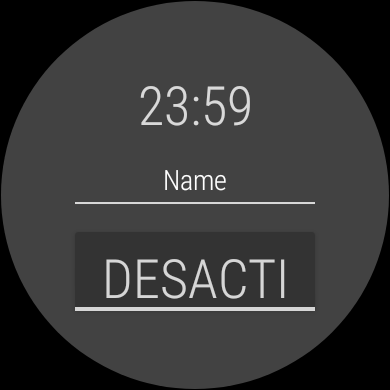
\includegraphics[width=\linewidth]{appActivity.png}
      \caption{Aplicación de gestión}
      \label{fig:uiActivity}
  \end{subfigure}
  \hfill
  \begin{subfigure}[b]{0.4\textwidth}
      \centering
      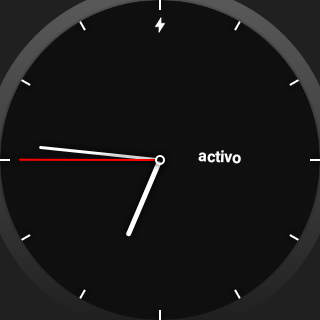
\includegraphics[width=\linewidth]{appWatchface.png}
      \caption{\textit{Watchface}}
      \label{fig:uiWatchface}
  \end{subfigure}
  \caption{\label{fig:ifell:UI} Interfaz de usuario de iFell}
\iffalse
\subfloat{\label{fig:uiActivity} Aplicación de gestión}{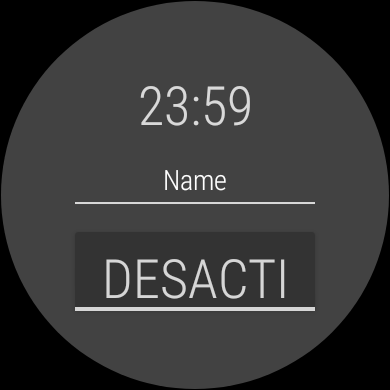
\includegraphics[width=0.4\linewidth]{appActivity.png}}
     \caption{\label{fig:uiApps} Interfaces de usuario}
     \hfill
\subfloat{\label{fig:uiWatchface} Watchface}{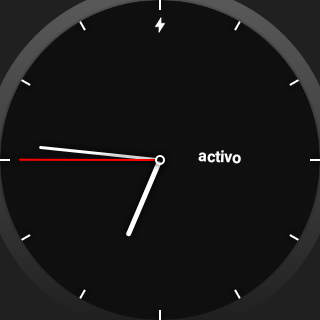
\includegraphics[width=0.4\linewidth]{appWatchface.png}}
\fi
\end{figure}


La aplicación toma forma de un objeto cotidiano e interactúa con el usuario utilizando un concepto conocido para este: un reloj digital. La única información que se muestra al usuario es la hora (adicionalmente el propio sistema operativo sobreimprime indicaciones de batería baja, ausencia de conexión a internet y existencia de notificaciones de otros servicios y aplicaciones). De esta forma, para el usuario, el dispositivo se convierte en un objeto conocido con un uso muy extendido que de forma adicional a su función tradicional realiza el proceso de detección de caídas.

En esta aplicación se han reducido al máximo las interacciones requeridas por parte del usuario en todo momento, hasta el punto de no requerir ninguna. La aplicación funciona en todo momento como un reloj tradicional mostrando la hora de forma analógica mediante unas manecillas. En el caso de detectarse una caída o evento similar, emitirá de forma automática una serie de avisos visuales, acústicos y hápticos (según las capacidades del dispositivo sobre el que se ejecute) que podrán ser desactivados si se detecta actividad nuevamente. Aunque también existe la posibilidad de desactivarlos tocando la pantalla.

La segunda interfaz que provee la aplicación se encarga de las tareas de administración y configuración. Permite introducir un nombre del usuario y forzar el estado de funcionamiento de los servicios de captura y detección. Si bien ninguno de estos procesos es necesario para el funcionamiento, se ofrece para facilitar la puesta en marcha y prueba del sistema.

\subsection{Comunicación con el Servidor}


% ########################################

El desafío de consolidar en un sistema portable una aplicación autónoma de detección de caídas debe hacer frente a una serie de limitaciones.

\section{Desafíos}
\todo{esto son requisitos, movel al punto anterior} El objetivo de todo modelo de detección de eventos es lograr un sistema que consiga capturar la totalidad de las realizaciones del mismo con el menos número posible de falsos positivos. En otras palabras, buscamos un sistema con una especificidad y sensibilidad de 100\%\cite{Noury2007}. \todo{Añadir referencias a papers, comentarios sobre sensibilidad y especificidad}.

\subsection{Usabilidad}\todo{de nuevo un requisito, al apartado anterior}
El primer reto de toda aplicación es conseguir una experiencia de usuario adaptada al cliente final. De nada sirve lograr implementar una plataforma que cumpla perfectamente con todos los requisitos y objetivos funcionales si el producto resultante se utiliza.

\subsubsection{Público objetivo}
Como se ha mencionado en la introducción del trabajo, los daños relacionados con las caídas son una de las principales causas de mortaldad entre las personas mayores de 65 años \todo{cita requerida}. Es propio de este grupo de población la desafección por la tecnología y la carencia o desinterés por su uso. Esta condición ha de ser tenida en cuenta para el desarrollo de cualquier producto.

Las personas de edad avanzada suelen padecer así mismo de otras condiciones que pueden limitar su grado de movilidad, atención o memoria que impidan o reduzcan la posibilidad de adaptarse o incorporar nuevas rutinas. Los problemas motores y de percepción reducen notablemente la capacidad de mostrar información así como de interactuar con el usuario cuando se necesite una acción por su parte.

Se entiende por tanto que si se ha de realizar un producto para esta población, es requisito que sea lo menos obtrusivo posible \todo{de nuevo un requisito, al punto anterior}, siendo recomendable incorporar la funcionalidad a un objeto de uso cotidiano para evitar la modificación de rutinas o la reticencia a incorporar nuevos procesos o elementos en su vida diaria. La interfaz de usuario debe ser mínima, usando un lenguaje visual que resulte familiar alejado de los estándares de las aplicaciones modernas. Así mismo, reducir o eliminar los procesos de configuración y manipulación, con un sistema que funcione al salir de la caja \todo{mala traducción de \textit{out of the box}}.

\subsubsection{Localización}

Una de las decisiones con mayor impacto sobre la funcionalidad del prototipo es la elección de la posición del dispositivo de captura ya que influencia en gran medida a la capacidad de detección de caídas \cite{Kangas2008}. Diversos estudios muestran que el mejor lugar para posicionar un sistema de medición de la aceleración para detectar caídas es la cintura, seguida de la cabeza siendo posible también usar un medidor en la muñeca\cite{Chen2005, Kangas2008, Noury2007}. Si bien estos resultados se basan en el análisis de métodos analíticos basados en cotas, se desprende de ellos la actitud o posición del cuerpo es un buen indicador para la predicción de actividades, razón por la que realizar la captura en muñecas o tobillos, las extremidades más alejadas del tronco, sufren de mayores penalizaciones para conseguir buenas estimaciones.

Al optarse por un reloj o \textit{pulsera de actividad} como plataforma para la implementación las opciones para posicionar la unidad de medida quedan reducida a una: la muñeca.

\subsection{Conectividad}

Hasta la fecha, los sistemas de detección de caídas se basan en arquitecturas cliente servidor para disociar el módulo de cómputo del de captura y conseguir que el dispositivo a llevar en si sea del menor tamaño posible. Este acercamiento que permite solventar el problema que derivaría de tener que llevar un obtrusivo sistema sobre si añade el problema de la necesidad de un enlace o comunicación con el módulo de cálculo. Ganamos en usabilidad pero perdemos en portabilidad.\todo{Cita y referencias a sistemas comerciales}

El principal problema de la conectividad radica en el hecho de que a pérdida de comunicación entre ambos módulos deriva en un sistema con ninguna capacidad. El módulo de cálculo, privado de datos no es capaz de realizar ninguna detección. Por su parte el aparato de captura, por si mismo, no tiene capacidad alguna para realizar nada más que la lectura.

El sistema implementado opta por una arquitectura cliente-pesado y servidor ligero. El cliente tiene suficiente capacidad para realizar captura, cómputo y capacidad de alerta como para funcionar de forma aislada. El servidor realiza funciones de expansión de la capacidad de alerta de la plataforma, así como de distribución de actualizaciones o mejoras en modelos y parámetros, pero de ninguna manera resulta imprescindible para el funcionamiento del dispositivo portable. Este es el principio básico y director de este trabajo: implementar una plataforma autónoma de detección de caídas capaz de ejecutarse en un dispositibo vestible.


\section{Plataforma}
\todo{justificar cada una de estas decisiones}
Para el servidor optamos por una arquitectura de microservicios usando la plataforma de AWS Lambda con almacenamiento en S3

Para el dispositivo móvil usamos un reloj inteligente Fossil Sport con sistema operativo WearOS y por tanto compatible con el ecosistema Android.

El la generación, entrenamiento, análisis y evaluación de modelos se realiza usando Keras/Tensorflow corriendo en la plataforma Google Colab.

\section{Arquitectura}\label{desc_archi}
\warn{según la profe punto muy interesante, a pulir }

\subsection{Arquitectura del sistema}

\warn{hablando de AWS: (ver siguiente páraffo)}
Resumiendo la estructura del sistema, \textit{AWS S3} (\url{https://aws.amazon.com/es/s3/?c=ser&sec=srv}) es el sistema de almacenamiento de datos en la red. Un disco duro en la nube, escalable en capacidad y fácilmente accesible para poder recuperar los datos. \textit{AWS Lambda} (\url{https://aws.amazon.com/es/lambda/?c=ser&sec=srv}) permite implementar funciones de código y definir una serie de eventos para lanzar su ejecución, al formar parte del ecosistema AWS es fácil conectar estas funciones con el sistema S3 y API Gateway. Finalmente \textit{AWS API Gateway} permite definir unos puntos de entrada, o URLs que conformarán la API del servicio. Cuando una de estas direcciones URL es invocada, inmediatamente se ejecuta la 



\todo{show me the data!!! cómo llegamos a 3G?}
El valor de $A_{umbral}$ se obtiene experimentalmente gracias al análisis de los datos obtenidos. Se fija en $A_{umbral} = 3G$ que resulta un buen equilibrio ya que conseguimos una cantidad reducida de eventos manteniendo un nivel bajo\todo{citar trabajos y medidas. Bourke usa 3,5G, otros usan valores más altos, la mayoría de caídas tienen niveles instantáneos de SVTot superiores a 6G}.\todo{incluir trabajo estadístico de los datos de aceleración del dataset} \todo{incluir gráfica temporal explicativa del algoritmo}

Si se sobrepasa el umbral en $t=0$. El sistema envía instantáneamente al siguiente modelo las muestras entre $t=-225$ y $t=-25$ (4 segudnos previos al evento). En segundo plano sigue capturando muestras hasta $t=25$. Este segundo bloque de 50 muestras (un segundo centrado en el evento) se envía también a la siguiente etapa. La decisión de separar el envío de datos a la siguiente etapa está motivada por la reducción de la latencia del sistema y obtener una clasificación o resultado con la menor dilación posible.


\subsubsection{Modelo RNN}


El modelo predictivo, se basa en la capacidad de las redes RNN y particularmente las basadas en celdas LSTM y GRU para generar modelos predictivos de calidad para series temporales de señales estacionarias \cite{Qin2019}.




\figura{trainingModeloRNN}{fig:rnnTrainAlt}{Evolución de RMSE durante el entrenamiento}

\figura{prediction.png}{fig:prediccionAceleracion}{Predicción de la aceleración}

\paragraph*{Detección}

Este segundo bloque recibe por un lado la señal $SVTot(-25:25)$\todo{no es un formato aceptable, usar t-25, t-24, .... t+25 o algo que sea aceptable} del acelerómetro y por el segundo la predicción $\hat{SVTot}(-25:25)$ \todo{unificat nomenclatura!!!}. Para clasificar el evento como una caída, usaremos un umbral sobre el error de predicción del modelo recurrente. La métrica de error empleada es la \textit{Raíz del Error Cuadrático Medio} definida como: \[
RECM=\sqrt{1/T\sum_{t_1}^{t_2}|y-\hat{y}|^2 }
\]Donde $t_1 = -25$, $t_2 = 25$ y $T=t_2-t_1=50$.

Comparando el resultado del error obtenido con un nuevo umbral al que denominaremos umbral de detección $U_{d}$ obtendremos finalmente la clasificación del evento en \textit{Caída} o \textit{no-Caida}. Dicho umbral se obtiene de nuevo de forma experimental.

En este caso el valor utilizado se calcula mediante el análisis del RECM usado durante la validación del modelo durante el entrenamiento. \todo{mostrar valores}

